\documentclass[12pt]{article}
\usepackage[russian]{babel}
\usepackage{geometry}

\usepackage{graphicx} % вставка изображений
\usepackage{caption} % описание изображений

%различные цветовые модели
\usepackage[usenames]{color}
\usepackage[dvipsnames,table]{xcolor}
\usepackage{colortbl}

\usepackage{tikz}
\usetikzlibrary{shapes, arrows}
\usepackage{varwidth}
\usepackage{ifthen}

\usepackage{multicol} % вставка изображений в две колонки


%циклы foreach в tikz и создание переменных внутри этого окружения
\usepackage{pgffor}
\usepackage{pgfmath}

\usepackage{xifthen}

\usepackage{afterpage}

\usepackage{amssymb}
\usepackage{amsmath}

\usepackage{hyperref}

\usepackage[utf8]{inputenc}

\tikzstyle{connector} = [draw, -latex']
\tikzstyle{line} = [draw, -]
\tikzstyle{dashed} = [draw, -, dash pattern=on 5pt off 5pt]


\usepackage{listings}
\usepackage{listingsutf8}
\usepackage[T2A]{fontenc}
\newcommand{\listingsttfamily}{\usefont{T2A}{PTMono-TLF}{m}{n}}

\lstset{
	language=C,                % choose the language of the code
	numbers=left,                   % where to put the line-numbers
	stepnumber=1,                   % the step between two line-numbers.        
	numbersep=5pt,                  % how far the line-numbers are from the code
	backgroundcolor=\color{black},  % choose the background color. You must add \usepackage{color}
	commentstyle=\color{Gray},
	basicstyle=\listingsttfamily\color{Gray},
	keywordstyle=\color{BurntOrange},
	stringstyle=\color{YellowGreen},
	showspaces=false,               % show spaces adding particular underscores
	showstringspaces=false,         % underline spaces within strings
	showtabs=false,                 % show tabs within strings adding particular underscores
	tabsize=4,                      % sets default tabsize to 2 spaces
	captionpos=b,                   % sets the caption-position to bottom
	breaklines=true,                % sets automatic line breaking
	breakatwhitespace=true,         % sets if automatic breaks should only happen at whitespace
	title=\lstname, 
	inputencoding=utf8,                % show the filename of files included with \lstinputlisting;
	extendedchars=\true,
	keepspaces=true
}

\geometry{top=2cm, bottom=2cm, left=3cm, right=1.5cm}
\textheight=24cm
\textwidth=18cm
\flushbottom 

\oddsidemargin=0pt 
\topmargin=-1.5cm 
\parskip=0.25cm
\parindent=24pt 

\tolerance=2000 

\setcounter{secnumdepth}{0}

\begin{document}
	\begin{center}
		{\parskip=1cm
			МИНИСТЕРСТВО НАУКИ И ВЫСШЕГО ОБРАЗОВАНИЯ РОССИЙСКОЙ ФЕДЕРАЦИИ
			
			ФЕДЕРАЛЬНОЕ ГОСУДАРСТВЕННОЕ БЮДЖЕТНОЕ ОБРАЗОВАТЕЛЬНОЕ УЧРЕЖДЕНИЕ ВЫСШЕГО ОБРАЗОВАНИЯ
			
			{\bf«БЕЛГОРОДСКИЙ ГОСУДАРСТВЕННЫЙ ТЕХНОЛОГИЧЕСКИЙ УНИВЕРСИТЕТ им. В. Г. Шухова»\\(БГТУ им. В. Г. Шухова)}
			
			\begin{figure}[bh]
				\noindent\centering{
					
\includegraphics[width=100mm]{images/start_logo.png}
					\captionsetup{labelformat=empty}
				}
			\end{figure}
			Кафедра программного обеспечения вычислительной техники и автоматизированных систем
		}
		
		{\Large 
			\vspace{1cm}
			{\parskip=0.25cm 
				{\bf Лабораторная работа №3.2}
				
				по дисциплине: «Дискретная математика»

				по теме: {\bf Транзитивное замыкание отношения}
			}
		}
	\end{center}	
	\begin{flushleft}
		{\leftskip=10cm
			{\vspace{3cm} Выполнил/a: ст. группы ПВ-231}
			
			Чупахина София Александровна
			
			Проверил: Рязанов Юрий Дмитриевич
			
		}
	\end{flushleft}
	\begin{center}
		{\parskip=3cm Белгород, 2024}
	\end{center}
	\newpage
	
	\tableofcontents
	\newpage
	
	\subsection{Используемые библиотеки}
	\label{libraries}
	Перед выполнением лабораторной работы прикрепим к ней текст функций для работы с отношениями. Мы задали отношения как структуру и написали ряд функций, повторяющих объявленные над ними операции, для работы с ними в рамках лабораторной работы 3.1. 
	
	\lstinputlisting{../../ДИСКРЕТКА ЛАБА 3.1/bin_relations/bin_relation_definition_input_output.c} 
	\lstinputlisting{../../ДИСКРЕТКА ЛАБА 3.1/bin_relations/bin_relations_operations.c} 
	
	\newpage
	
	\subsection{Задание 1}
	\label{task1}
	{\bf Текст задания:} Написать программу для реализации следующего алгоритма вычисления транзитивного замыкания отношения $A$, построенного на множестве $M$:
	
	{\parskip=0.05cm
	Алгоритм 1.
	
	Вход: $A$ — отношение.
	
	Выход: $C$ — транзитивное замыкание отношения $A$.
	
	1. $C$ := $A$; $S$ := $A o A$.
	
	2. Пока $\overline{S \subseteq C}$ выполнять:
	
	{\hangindent=2cm \hangafter=-1 \noindent
	$C$ := $C \cup S$; $S$ := $S o A$.
	
	3. Конец алгоритма.
	}
	}
	
	Поскольку в прошлой лабораторной работе мы написали библиотеку для выполнения основных операций над отношениями, в число которых входит проверка включения (то есть проверка, является ли одно отношение нестрогим подмножеством другого), объединение и композиция, для нас не составит труда реализовать этот алгоритм:
	
	\lstinputlisting[firstline=4, lastline=12]{../programs/closures_relations.c} 
	
	\subsection{Задание 2}
	\label{task2}
	{\bf Текст задания:} Привести пример отношения $A$ на множестве $M = \{1, 2, 3, 4, 5, 6, 7, 8, 9, 10\}$, при обработке которого алгоритмом 1 композиция выполнится не большее количество раз, чем при обработке любого другого отношения на множестве М.
	
	Сколько раз выполнится композиция при обработке отношения $A$? Проверить экспериментально.
	
	Определить, какое количество операций сравнения выполнится при обработке отношения $A$.
	
	Если перед нами стоит задача найти такое отношение $A$, при обработке которого алгоритмом отношения 1 композиция выполнится {\bf не большее} количество раз, чем при обработке любых других отношений, значит, количество выполненных композиций для обработки отношения $A$ должно быть {\bf наименьшим}. Логично предположить, что оно будет наименьшим, когда для отношения $A$ не нужно искать транзитивное замыкание: отношение уже транзитивно, и алгоритм прекратит выполнение сразу же, как только сможет это распознать. 
	
	Сколько именно композиций потребуется выполнить для его обработки? Отношение транзитивно, если при вхождении в него пар вида $(x, z)$ и $(z, y)$ в него также будет входить пара вида $(x, y)$. Значит, квадрат отношения $A$, содержащий в себе все такие <<результирующие>> пары, будет входить в исходное отношение. Для проверки данным алгоритмом факта транзитивности исходного отношения достаточно выполнить композицию {\bf один раз}, чтобы получить его квадрат. Следом за этим шагом условие цикла возвращает ложь (вспомогательное отношение $S$ является подмножеством отношения $C$, которое на данном шаге равно исходному), и функция возвращает отношение $C$, равное отношению $A$.
	
	Как пример транзитивного отношения можем рассмотреть множество, образованное декартовым произведением непересекающихся подмножеств множества $M$. Если $x$-элементы всех пар берутся из некоторого множества $X$ и $y$-элементы всех пар берутся из некоторого множества $Y$, и при этом $X \cap Y = \emptyset$, то не найдется двух пар вида $(x, z)$ и $(z, y)$, ведь это значило бы, что $z \in X$ и $z \in Y$. А когда такие пары отсутствуют, отношение можно считать транзитивным: условие $xRz \& zRy \to \overline{xRy}$ не будет нарушаться, ведь оно всегда истинно, если импликация следует из лжи.
	
	Итак, зададим отношение $A$ как $\{1, 2, 4, 5, 7\} \times \{3, 8, 10\}$. Перед тем, как начать с ним работать, создадим модифицированный вариант функции transitive\_closure\_algorithm1, который, помимо возвращения транзитивного замыкания отношения $A$, сохраняет по указанному адресу число --- количество выполненных композиций (поскольку количество композиций требуется найти экспериментально). В теле main создадим отношение $A$, переменные для хранения количества выполненных сравнений и композиций, а затем вызовем модифицированную функцию для получения транзитивного замыкания отношения A. Результаты работы --- матрицу транзитивного замыкания и количество композиций --- выведем на экран.
	
	\lstinputlisting[linerange={38-48, 80-93, 134}]{../programs/closures_relations.c} 
	
	\begin{figure}[h]
		\noindent\centering{
			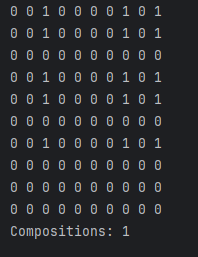
\includegraphics[width=60mm]{images/output1.png}
			\caption{Вывод результата работы алгоритма 1 на отношении с минимально возможным количеством композиций}
		}
	\end{figure}
	
	Как видим, была выполнена всего одна композиция. 
	
	Перейдем к вопросу вычисления количества сравнений (его не нужно подтверждать экспериментально). Для этого разберемся, какие вообще функции использует этот алгоритм и сколько сравнений содержит каждая из них. 
	
	Создание переменной-структуры и присвоение ей значения не требует сравнений. 
	
	Операция композиции (слегка измененная по сравнению с вариантом в лабораторной работе 3.1) содержит в себе два вложенных цикла, задающих элементы пары i и j в диапазоне от 1 до $|M|$; внутри располагается проверка на то, входит ли рассматриваемая пара в первое отношение (это как раз и есть операция сравнения), после чего i-тая строка результирующего отношения находится как побитовое <<или>> ее текущего значения с j-той строкой второго отношения. Побитовые операции, в свою очередь, производятся мгновенно (имеют нулевой порядок функции временной сложности) и не требуют операций сравнения. Однако следует помнить, что перебор значений переменной внешнего цикла приведет к выполнению $|M|+1$ операций сравнения ($M$ сравнений, проверяющих, не вышла ли переменная за рамки диапазона, в ходе которых условие продолжения цикла истинно, и 1 сравнение, когда оно оказывается ложным), а перебор значений внутреннего цикла --- к выполнению $(|M|+1)*|M|$ сравнений (по $|M|+1$ сравнений при возрастании переменной внутреннего цикла, которое будет производиться $|M|$ раз). То есть композиция приводит к выполнению $|M|^2 + |M|+1 + (|M|+1)*|M|$ = $|M|^2 + (|M|+1)*(|M|+1)$ = $|M|^2 + (|M|+1)^2$ операций сравнения. 
	
	Операция проверки вхождения одного отношения в другое содержит в себе один цикл, перебирающий номера строк от 1 до $|M|$ (в нашем случае мощности множеств, на которых построены отношения, одинаковы), и анализирует, является ли одна строка вхождением в другую, с помощью побитовых операций и одной операции сравнения. То есть каждое применение операции сравнения приводит к выполнению $|M|$ операций сравнения непосредственно в ходе выполнения, плюс $|M| + 1$ операций выполняются в ходе перебора значений цикла. 
	
	Наконец, операция объединения также состоит из одного цикла, перебирающего номера строк от 1 до $|M|$, и строка результирующей матрицы с текущим номером находится как результат побитового <<или>> соответствующих строк матриц, над которыми проводится объединение. Это действие само по себе не содержит операций сравнения, но $|M|+1$ операций сравнения выполняются при переборе значений цикла.
	
	Заметим, что операции композиции, объединения и проверки на вхождение выполняются по одному разу на каждую итерацию цикла, однако помимо этого, композиция один раз выполняется до запуска цикла, а проверка на вхождение --- и тогда, когда условие продолжения цикла обращается в ложь и следующая итерация не запускается. То есть всего композиций и проверок на вхождение происходит k+1, где k --- количество итераций цикла, а количество операций сравнения за все время выполнения алгоритма будет равно ($|M|^2$ + $(|M|+1)^2$ + $|M|$ + $|M|+1$) * (k+1) + ($|M|+1$) * k. 
	
	В случае, когда отношение $A$ транзитивно изначально, цикл не будет выполняться ни разу, и количество операций сравнения можно вычислить как ($|M|^2$ + $(|M|+1)^2$ + $|M|$ + $|M|+1$) * (0+1) + ($|M|+1$) * 0 = ($|M|^2$ + $(|M|+1)^2$ + $|M|$ + $|M|+1$) * 1 = $|M|^2$ + $(|M|+1)^2$ + $|M|$ + $|M|+1$ = $10^2$ + $(10+1)^2$ + 10 + 10+1 = 100 + 121 + 10 + 11 = 242.
	
	\subsection{Задание 3}
	\label{task3}
	{\bf Текст задания:} Привести пример отношения $A$ на множестве $M = \{1, 2, 3, 4, 5, 6, 7, 8, 9, 10\}$, при обработке которого алгоритмом 1 композиция выполнится не меньшее количество раз, чем при обработке любого другого отношения на множестве М.
	
	Сколько раз выполнится композиция при обработке отношения $A$? Проверить экспериментально.
	
	Определить, какое количество операций сравнения выполнится при обработке отношения $A$.

	Если перед нами стоит задача найти такое отношение $A$, при обработке которого алгоритмом отношения 1 композиция выполнится {\bf не меньшее} количество раз, чем при обработке любых других отношений, значит, количество выполненных композиций для обработки отношения $A$ должно быть {\bf наибольшим}. Что вообще нужно, чтобы построить транзитивное замыкание отношения? Задача сводится к тому, чтобы включить в исходное отношение все пары из элементов, которые в графе исходного отношения соединены цепочкой дуг любой длины, то есть принадлежат любому из отношений $A^{2}$, $A^3$, ..., $A^{|M|}$, где $M$ --- мощность множества, на котором построено отношение. Текущий алгоритм же, по сути, создает отношение $C$, которое изначально равно исходному $A$, и вспомогательное отношение $S$, которое изначально равно $A^2$. С каждой итерацией цикла отношение $C$ объединяется с текущим отношением $S$, а потом выполняется композиция множества $S$ с $A$, то есть $S$ становится равно $A^3$, ..., $A^{|M|}$. Получается, алгоритм сводится к постепенному добавлению в результирующее отношение пар, входящих в степени исходного отношения по возрастанию, то есть пара из отношения $A$ в максимальной степени будет добавлена последней, и до ее добавления алгоритм не завершится. Тогда и количество выполненных композиций будет наибольшим, когда в отношении $A$ есть некая пара, элементы которой связаны цепочкой дуг длиной $|M|$. Эта пара будет принадлежать множеству $A^{|M|}$, в нашем случае $A^{10}$, и транзитивное замыкание будет завершенным только после ее добавления после {\bf десяти} композиций.
	
	Как пример отношения, содержащего такую пару, можем рассмотреть отношение, состоящее только из следующих пар: $\{1, 2\}$, $\{2, 3\}$, $\{3, 4\}$, $\{4, 5\}$, $\{5, 6\}$, $\{6, 7\}$, $\{7, 8\}$, $\{8, 9\}$, $\{9, 10\}$, $\{10, 1\}$. Пара $\{1, 1\}$ в него не входит, и сам с собой элемент 1 соединен цепочкой из 10 дуг. Зададим такое множество в теле функции main и применим к нему экспериментальную версию алгоритма 1.
	
	\lstinputlisting[linerange={80, 101-109, 134}]{../programs/closures_relations.c} 
	
	\newpage
	
	\begin{figure}[h]
		\noindent\centering{
			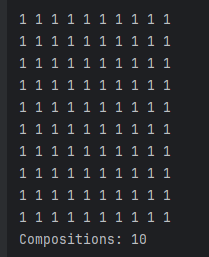
\includegraphics[width=60mm]{images/output2.png}
			\caption{Вывод результата работы алгоритма 1 на отношении с максимально возможным количеством композиций}
		}
	\end{figure}
	
	Как видим, было выполнено ровно десять композиций. 
	
	Переходя к задаче подсчета количества сравнений, мы можем воспользоваться формулой, выведенной в задании 2: ($|M|^2$ + $(|M|+1)^2$ + $|M|$ + $|M|+1$) * (k+1) + ($|M|+1$) * k. Остается только найти K для этого случая. В начале выполнения алгоритма будущее транзитивное замыкание, если рассматривать его как объединение степеней отношения $A$, содержит в себе только первую степень, и с каждой итерацией цикла максимальная степень будет увеличиваться на 1. До 10 она дойдет за 9 итераций цикла, и количество сравнений будет равно ($|M|^2$ + $(|M|+1)^2$ + $|M|$ + $|M|+1$) * (9+1) + ($|M|+1$) * 9 = 10 * ($|M|^2$ + $(|M|+1)^2$ + $|M|$ + $|M|+1$) + 9 * ($|M|+1$) = 10 * ($10^2$ + $(10+1)^2$ + $10$ + $10+1$) + 9 * ($10+1$) = 10 * (100 + 121 + 10 + 11) + 9 * 11 = 10 * 242 + 99 = 2420 + 99 = 2519.
	
	\subsection{Задание 4}
	\label{task4}
	{\bf Текст задания:} Написать программу для реализации следующего алгоритма вычисления транзитивного замыкания отношения $A$, построенного на множестве $M$:
	
	{\parskip=0.05cm
	Алгоритм 2.
	
	Вход: $A$ — отношение.
	
	Выход: $C$ — транзитивное замыкание отношения $A$.
	
	1. $C$ := $A$; $C2$ := $C o C$.
	
	2. Пока $\overline{C2 \subseteq C}$ выполнять:
	{\hangindent=2cm \hangafter=-1 \noindent
	$C$ := $C \cup C2$; $С2$ := $C o C$.
	
	3. Конец алгоритма.
	}
	}
	
	Этот алгоритм структурно похож на алгоритм 1: все, что требуется, чтобы получить его из первого --- замена нескольких переменных. Так что он так же легко поддается программной реализации:
	\lstinputlisting[firstline=13, lastline=21]{../programs/closures_relations.c} 
	
	\subsection{Задание 5}
	\label{task5}
	{\bf Текст задания:} Привести пример отношения $A$ на множестве $M = \{1, 2, 3, 4, 5, 6, 7, 8, 9, 10\}$, при обработке которого алгоритмом 2 композиция выполнится не большее количество раз, чем при обработке любого другого отношения на множестве М.
	
	Сколько раз выполнится композиция при обработке отношения $A$? Проверить экспериментально.
	
	Определить, какое количество операций сравнения выполнится при обработке отношения $A$.
	
	Первые шаги данного алгоритма очень похожи на первые шаги алгоритма 1. Создается отношение для записи будущего транзитивного замыкания, изначально равное исходному отношению $A$, и вспомогательное отношение, равное квадрату исходного отношения, $A^2$. Как мы выяснили в ходе выполнения задания 2, если квадрат исходного отношения входит в само отношение $A$, то $A$ уже транзитивно, и достаточно выполнить {\bf одну} композицию для получения квадрата отношения $A$ и сравнения его с исходным отношением. Значит, как отношение, при обработке которого будет совершено наименьшее количество композиций, мы можем взять заведомо транзитивное отношение из задания 2. 
	
	Проверим это экспериментально. Внесем в функцию алгоритма 2 такие же изменения для отслеживания количества совершенных композиций и сохранения этого количества во внешнюю переменную. Затем для уже полученного в теле main транзитивного множества запустим этот алгоритм, выведя результат выполнения и количество композиций на экран.
	
	\lstinputlisting[linerange={49-59, 80-88, 95-98, 134}]{../programs/closures_relations.c} 

	
	\begin{figure}[h]
		\noindent\centering{
			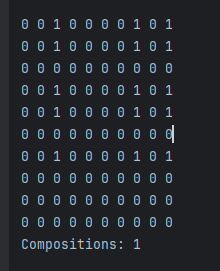
\includegraphics[width=60mm]{images/output3.png}
			\caption{Вывод результата работы алгоритма 2 на отношении с минимально возможным количеством композиций}
		}
	\end{figure}
	
	Как видим, была выполнена всего одна композиция, как и для похожего случая с применением алгоритма 1. 
	
	Перейдем к вычислению количества операций сравнения в ходе выполнения этого алгоритма. Для него, как и для алгоритма 1, справедливо, что для одной итерации цикла выполняется по одной операции композиции, объединения и проверки на вхождение; также верно, что одна операция композиции выполняется перед запуском цикла, а одна операция проверки на вхождение --- в ходе проверки условия в момент выхода из цикла. Получим все ту же формулу для вычисления количества операций сравнения: ($|M|^2$ + $(|M|+1)^2$ + $|M|$ + $|M|+1$) * (k+1) + ($|M|+1$) * k, где k --- количество итераций цикла. В этом случае k = 0, и ($|M|^2$ + $(|M|+1)^2$ + $|M|$ + $|M|+1$) * (0+1) + ($|M|+1$) * 0 = ($|M|^2$ + $(|M|+1)^2$ + $|M|$ + $|M|+1$) * 1 = $|M|^2$ + $(|M|+1)^2$ + $|M|$ + $|M|+1$ = $10^2$ + $(10+1)^2$ + 10 + 10 + 1. = 100 + 121 + 10 + 11 = 242.
		
	\subsection{Задание 6}
	\label{task6}
	{\bf Текст задания:} Привести пример отношения $A$ на множестве $M = \{1, 2, 3, 4, 5, 6, 7, 8, 9, 10\}$, при обработке которого алгоритмом 2 композиция выполнится не меньшее количество раз, чем при обработке любого другого отношения на множестве М.
	
	Сколько раз выполнится композиция при обработке отношения $A$? Проверить экспериментально.
	
	Определить, какое количество операций сравнения выполнится при обработке отношения $A$.
	
	По сути, этот алгоритм также представляет из себя постепенное повышение степени вспомогательного отношения $C2$ и его объединение с формируемым транзитивным замыканием $C$ на каждой итерации цикла, однако более быстрое. Рассмотрим значения отношений $C2$ и $C$ на первых нескольких итерациях, если условие продолжения цикла остается истинным:
	{\parskip=0.05cm
		\begin{description}
			\item[0.] $C$ = $A$; \\
			$C2$ = $C o C$ = $A o A$ = $A^2$;
			
			\item[1.] $C$ = $C \cup C2$ = $A \cup A^2$; \\
			$C2$ = $C o C$ = $(A \cup A^2) o (A \cup A^2)$ = $A^2 \cup A^3 \cup A^3 \cup A^4$ = $A^2 \cup A^3 \cup A^4$;
			
			\item[2.] $C$ = $(C \cup C2)$ = $(A \cup A^2) \cup (A^2 \cup A^3 \cup A^4)$ = $A \cup A^2 \cup A^3 \cup A^4$; \\
			$C2$ = $C o C$ = $(A \cup A^2 \cup A^3 \cup A^4) o (A \cup A^2 \cup A^3 \cup A^4)$ = ... = $A^2 \cup A^3 \cup A^4 \cup A^5 \cup A^6 \cup A^7 \cup A^8$;
			
			\item[3.] $C$ = $(C \cup C2)$ = $(A \cup A^2 \cup A^3 \cup A^4) \cup (A^2 \cup A^3 \cup ... \cup A^8)$ = $A \cup A^2 \cup ... \cup A^8$; \\
			$C2$ = $C o C$ = $(A \cup A^2 \cup ... \cup A^8) o (A \cup A^2 \cup ... \cup A^8)$ = ... = $A^2 \cup A^3 \cup ... \cup A^{16}$;	
		\end{description}
	}
	То есть, хотя вспомогательное отношение $C2$ представляет собой уже не максимальную для текущей итерации степень отношения $A$, а объединение степеней вплоть до максимальной, а сама максимальная степень с каждой итерацией не возрастает на 1, а увеличивается в 2 раза, одно остается неизменным: максимальная степень отношения $A$ включается в результирующее замыкание последней, в самом конце выполнения алгоритма. Значит, для наибольшего количества композиций в транзитивное замыкание должна входить пара, принадлежащая максимально возможной степени, $A^{|M|}$ ($A^{10}$ в нашем случае). Для этого два элемента в графе исходного отношения должны быть связаны цепочкой из $|M|$, 10 узлов. В таком случае, поскольку максимальная степень как вспомогательного отношения $C2$, так и результирующего отношения $C$ возрастает в 2 раза с каждой итерацией, мы сможем отследить, сколько потребуется композиций для включения в результирующее отношение степени $A^{10}$. Перед началом цикла, на <<нулевой>> итерации, максимальная степень результирующего отношения равна 1, и на этом шаге уже совершается композиция для задания стартового значения вспомогательного. На первой итерации максимальная степень результирующего равна 2, на второй --- 4, на третьей --- 8, и только на четвертой она достигнет 16 и перешагнет значение 10. Каждая итерация прибавит 1 к количеству совершенных композиций (за их счет меняется значение вспомогательного отношения), и всего их количество будет равно {\bf пяти}.
	
	Проверим это на практике, применив экспериментальную версию алгоритма 2 ко множеству из задания 3, в графе которого элемент 1 соединен с собой цепочкой из 10 дуг.
	
	\lstinputlisting[linerange={80, 101-104, 111-114, 134}]{../programs/closures_relations.c} 

	
	\begin{figure}[h]
		\noindent\centering{
			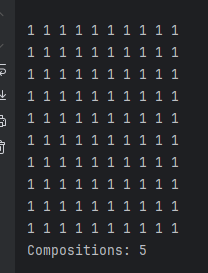
\includegraphics[width=60mm]{images/output4.png}
			\caption{Вывод результата работы алгоритма 2 на отношении с максимально возможным количеством композиций}
		}
	\end{figure}
	
	Результаты эксперимента сошлись с теоретическими рассуждениями: было выполнено ровно 5 композиций. 
	
	Для вычисления количества сравнений воспользуемся уже знакомой формулой ($|M|^2$ + $(|M|+1)^2$ + $|M|$ + $|M|+1$) * (k+1) + ($|M|+1$) * k. Осталось только вычислить k. Поскольку в этом алгоритме старшая степень в результирующем отношении увеличивается в 2 раза с каждой итерацией, количество итераций, которые понадобятся, чтобы достичь некоторой степени n, можно вычислить как $k$ = $\lceil log_2{n}\rceil$. В нашем случае $k$ = $\lceil log_2{10}\rceil$ = $\lceil3.322\rceil$ = 4. Таким образом, количество операций сравнения в ходе выполнения этого алгоритма равно ($|M|^2$ + $(|M|+1)^2$ + $|M|$ + $|M|+1$) * (4+1) + ($|M|+1$) * 4 = 5 * ($|M|^2$ + $(|M|+1)^2$ + $|M|$ + $|M|+1$) + 4 * ($|M|+1$) = 5 * ($10^2$ + $(10+1)^2$ + $10$ + $10+1$) + 4 * ($10+1$) = 5 * (100 + 121 + 10 + 11) + 4 * 11 = 5 * 242 + 44 = 1210 + 44 = 1254.
	
	\subsection{Задание 7}
	\label{task7}
	{\bf Текст задания:} Написать программу для реализации следующего алгоритма вычисления транзитивного замыкания отношения $A$, построенного на множестве $M$:
	
	{\parskip=0.05cm
	Алгоритм 3.
	
	Вход: $A$ — отношение.
	
	Выход: $C$ — транзитивное замыкание отношения $A$.
	
	1. $C$ := $A$.
	
	2. Для всех $z \in M$ выполнить:
	
	{\hangindent=2cm \hangafter=-1 \noindent
	Для всех $x \in M$ выполнить:
	
	{\hangindent=3.5cm \hangafter=-1 \noindent
	Если $(x, z) \in C$ то 
	
	{\hangindent=5cm \hangafter=-1 \noindent
	Для всех $y \in M$ выполнить:
	
	{\hangindent=6.5cm \hangafter=-1 \noindent
	Если $(z, y) \in C$ то $C$ := $C \cup \{(x, y)\}$.
	
	3. Конец алгоритма.
	}
	}
	}
	}
	}
	
	Этот алгоритм также легко поддается программной реализации; в отличие от предыдущих, он не требует использования функций из <<библиотеки>> для работы над отношениями:
	\lstinputlisting[firstline=22, lastline=36]{../programs/closures_relations.c} 
	
	\subsection{Задание 8}
	\label{task8}
	{\bf Текст задания:} Привести пример отношения $A$ на множестве $M = \{1, 2, 3, 4, 5, 6, 7, 8, 9, 10\}$, при обработке которого алгоритмом 3 количество операций сравнения выполнится не большее количество раз, чем при обработке любого другого отношения на множестве $M$.
	
	Определить, какое количество операций сравнения выполнится при обработке отношения $A$. Проверить экспериментально.
	
	Алгоритм 3 построен следующим образом: внутри двух вложенных циклов, задающих элементы $z$ и $x$ текущей тройки в диапазоне от 1 до $|M|$, располагается условная конструкция, проверяющая, входит ли в формируемое транзитивное замыкание пара $(x, z)$ (соответственно, она содержит в себе операцию сравнения). Если это так, то запускается еще один цикл, задающий элемент $y$ тройки, и для каждого у в диапазоне от 1 до $|M|$ еще одна условная конструкция с операцией сравнения проверяет, входит ли в отношение пара $(z, y)$. Если да, в него включается и пара $(x, y)$. При этом не стоит забывать, что сравнение производится в ходе перебора значений $z$, $x$, $y$, в ходе проверки, удовлетворяют ли они до сих пор условиям и стоит ли продолжать перебор.
	
	Первая условная конструкция, вложенная в два цикла, выполняется независимо от значения текущей пары элементов $x$ и $z$. Конструкция, вложенная в цикл, перебирающий значения $y$, выполняется лишь тогда, когда $(x, z) \in C$. Значит, для того, чтобы количество операций сравнения было не большим, чем при обработке любого другого отношения на множестве $M$, для искомого значения количество операций сравнения должно быть {\bf наименьшим}, а для этого нужно найти отношение, для которого условие $(x, z) \in C$ выполняется как можно меньшее количество раз. Таким отношением будет пустое отношение: если в $A$ не входит ни одна пара, не найдется таких $x$ и $z$, чтобы выполнялось $(x, z) \in C$. В таком случае будет выполнено только по одной операции сравнения на каждую пару $x$ и $z$ (количество таких пар равно $|M|^2$ = $10^2$ = 100), плюс по 11 сравнений на каждое из значений $z$ (10 раз, когда условие цикла возвращало истину и значения не выходят за рамки указанного диапазона, и 1 раз, когда условие цикла возвращало ложь и цикл прекращает выполнение) и 10*11 сравнений на каждое из значений $x$ (пока $x$ возрастает в рамках указанного диапазона, выполнится 11 сравнений, и так будет повторяться для 10 значений $z$). Итого будет выполнено 100+11+10*11 = 221 сравнение.
	
	Проверим это экспериментально, модифицируя алгоритм 3 добавлением в него счетчика сравнений (при каждом сравнении увеличивается на 1 переменная по адресу, переданному как аргумент) Необходимо учесть: 1) увеличение счетчика на 1 {\bf перед} каждой из условных конструкций, 2) увеличение счетчика после каждой итерации цикла, вместе с увеличением переменной цикла, 3) однократное увеличение счетчика перед каждым циклом, чтобы нивелировать тот факт, что рано или поздно произойдет сравнение условия цикла, которое вернет ложь, и оно не будет учтено увеличением счетчика в пункте 2. Затем создадим в теле main пустое отношение и внешний счетчик сравнений и применив к ним модифицированный алгоритм 3.
	
	\lstinputlisting[linerange={60-80, 116-122, 134}]{../programs/closures_relations.c} 
	
	\begin{figure}[h]
		\noindent\centering{
			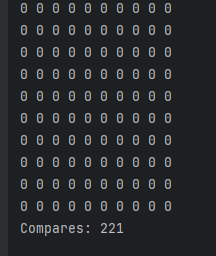
\includegraphics[width=60mm]{images/output5.png}
			\caption{Вывод результата работы алгоритма 3 на отношении с минимально возможным количеством сравнений}
		}
	\end{figure}
	
	Эксперимент подтверждает, что количество сравнений при обработке этим алгоритмом пустого отношения равно 221.
	
	\subsection{Задание 9}
	\label{task9}
	{\bf Текст задания:} Привести пример отношения $A$ на множестве $M = \{1, 2, 3, 4, 5, 6, 7, 8, 9, 10\}$, при обработке которого алгоритмом 3 количество операций сравнения выполнится не меньшее количество раз, чем при обработке любого другого отношения на множестве $M$.

	Определить, какое количество операций сравнения выполнится при обработке отношения $A$. Проверить экспериментально.
	
	Умозаключения в задании 8 могут быть применимы и здесь с обратным выводом: для того, чтобы количество операций сравнения было не меньшим, чем при обработке любого другого отношения на множестве $M$, для искомого значения количество операций сравнения должно быть {\bf наибольшим}, а для этого нужно найти отношение, для которого условие $(x, z) \in C$ выполняется как можно большее количество раз. Таким отношением будет универсальное отношение: если в $A$ входят все возможные пары, для каждого $x$ и $z$ в диапазоне от 1 до $|M|$ будет выполняться условие $(x, z) \in C$. В таком случае, помимо того, что будет выполнено по одной операции сравнения на каждую пару $x$ и $z$, будет выполнено по операции сравнения на каждую тройку x, z, y. Количество пар $x$ и $z$ равно $|M|^2$ = $10^2$ = 100, а количество троек $x$, $z$, $y$ равно $|M|^3$ = 1000. Не стоит забывать про 11 операций сравнения на перебор переменной $z$, 10*11 --- на перебор переменной $x$, и 10*10*11 --- на перебор переменной $y$. Всего операций сравнения будет выполнено 1000 + 100 + 11 + 10*11 + 10*10*11 = 1000 + 100 + 11 + 110 + 1100 = 2221.
	
	Проверим это экспериментально, создав в теле main универсальное отношение и внешний счетчик сравнений и применив к ним модифицированный алгоритм 3.
	
	\lstinputlisting[linerange={80, 123-134}]{../programs/closures_relations.c} 
	
	\newpage
	
	\begin{figure}[h]
		\noindent\centering{
			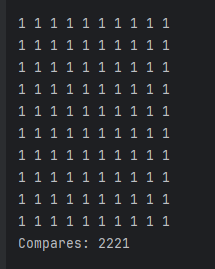
\includegraphics[width=60mm]{images/output6.png}
			\caption{Вывод результата работы алгоритма 3 на отношении с максимально возможным количеством сравнений}
		}
	\end{figure}
	
	Эксперимент подтверждает, что количество сравнений при обработке этим алгоритмом универсального отношения равно 2221.
	
	\subsection{Задание 10}
	\label{tas10}
	{\bf Текст задания:} Определить порядок функции временной сложности алгоритмов вычисления транзитивного замыкания.
	
	Мы уже рассматривали так или иначе операции, выполняемые в ходе работы всех трех алгоритмов. Для первого алгоритма это:
	\begin{itemize}
		\item[1.] Композиция: два вложенных цикла с перебором значений переменных от 1 до $|M|$ и последующим изменением строк результирующей матрицы отношения с помощью побитовых операций: порядок функции временной сложности равен $O(n^2)$,
		\item[2.] Проверка на включение одного отношения в другое: цикл с перебором значений переменной от 1 до $|M|$ и последующим сравнением строк двух матриц отношений с помощью побитовых операций: порядок функции временной сложности равен $O(n)$,
		\item[3.] Объединение: цикл с перебором значений переменной от 1 до $|M|$ и последующим получением строки результирующей матрицы отношения с помощью побитовых операций: порядок функции временной сложности равен $O(n)$.
	\end{itemize}
	В лучшем случае, когда поданное на вход отношение $A$ уже транзитивно, цикл не будет выполняться ни разу, и будут лишь единожды выполнены операции сравнения и композиции. Тогда порядок функции временной сложности алгоритма составит $O(n^2)$ (будет равен порядку функции временной сложности композиции, он является наибольшим среди ПФВС других операций). В худшем случае, когда в транзитивное замыкание необходимо включить пару, принадлежащую отношению $A^{|M|}$, будет выполнено максимальное число итераций цикла --- $|M|$ раз. Порядок функции временной сложности всего алгоритма в таком случае будет равен $O(n^3)$.

	Для второго алгоритма список операций будет в точности повторять первый:
	\begin{itemize}
		\item[1.] Композиция: два вложенных цикла с перебором значений переменных от 1 до $|M|$ и последующим изменением строк результирующей матрицы отношения с помощью побитовых операций: порядок функции временной сложности равен $O(n^2)$,
		\item[2.] Проверка на включение одного отношения в другое: цикл с перебором значений переменной от 1 до $|M|$ и последующим сравнением строк двух матриц отношений с помощью побитовых операций: порядок функции временной сложности равен $O(n)$,
		\item[3.] Объединение: цикл с перебором значений переменной от 1 до $|M|$ и последующим получением строки результирующей матрицы отношения с помощью побитовых операций: порядок функции временной сложности равен $O(n)$.
	\end{itemize}
	В лучшем случае, когда поданное на вход отношение $A$ уже транзитивно, цикл также не будет выполняться, и будут лишь единожды выполнены операции сравнения и композиции. Порядок функции временной сложности алгоритма для такого случая также составит $O(n^2)$. В худшем случае, когда в транзитивное замыкание необходимо включить пару, принадлежащую отношению $A^{|M|}$, будет выполнено максимальное число итераций цикла, равное $\lceil log_2{n}\rceil$ раз. Порядок временной сложности всего алгоритма равен $O(n^2log_2{n})$.
	
	Для третьего алгоритма не используются никакие операции, порядок функции временной сложности которых требовалось бы анализировать отдельно. Алгоритм использует три вложенных цикла с перебором значений переменных от 1 до $|M|$, однако третий запускается только в случае, когда пара, состоящая из первых двух переменных, входит в отношение $A$. В лучшем случае, когда отношение $A$ пустое и третий цикл не будет запущен ни разу, порядок функции временной сложности алгоритма будет равен $O(n^2)$. И наоборот, в худшем случае, когда отношение $A$ универсально и каждая пара переменных двух первых циклов приводит к запуску третьего, порядок функции временной сложности алгоритма будет равен $O(n^3)$.
	
	{\bf Вывод:} Замыкание $C_S$ бинарного отношения $A$ по признаку $S$ --- отношение, которое обладает признаком S, содержит в себе отношение $A$ и имеет при этом минимально возможную мощность. Для получения замыканий по некоторым свойствам, например, рефлексивности и симметричности, достаточно добавить быстро находимые недостающие элементы в исходное отношение. Для других свойств --- антирефлексивности, к примеру --- можно сразу сказать, что составить замыкание невозможно, если исходное отношение изначально не обладает этим свойством: ведь для этого придется убирать из него элементы, и тогда исходное отношение не будет входить в замыкание. Наиболее сложный случай --- замыкание по свойству транзитивности. Нельзя в один этап найти и добавить недостающие элементы: при их добавлении образуются новые пары вида $(x, z)$ и $(z, y)$, которые также необходимо учесть и добавить. В ходе лабораторной работы рассмотрели три основных алгоритма для получения транзитивных замыканий, проанализировали количество операций в некоторых экстремальных случаях для каждого из них и определили их порядок функции временной сложности.
	 
\end{document}	\label{subpart2_3}
